\documentclass[11pt]{article}
\usepackage{graphicx} % Required for inserting images
\usepackage{graphics}
\usepackage{geometry}
\usepackage{hyperref}
\usepackage{fontawesome5}
\geometry{
 a4paper,
 left=3cm,
 right=3cm,
 top=3cm,
 bottom=3cm
}

\title{
    Large Language Models Evaluation\\
    \vspace{1em}
    \small{\normalfont \href{https://github.com/tsounack/LLM_evaluation_pipeline}{https://github.com/tsounack/LLM\_evaluation\_pipeline}
    }
}
\author{Thomas Sounack}
\date{March 2024}


\begin{document}

\maketitle

\tableofcontents

\newpage

\section{Pipeline Design Overview}

Before running experiments, we can start by designing a pipeline to perform model inference. In addition to the benefit of familiarizing ourselves with the provided code, there are several objectives that this new pipeline will aim to achieve.

\begin{itemize}
    \item Build a modular back-end code base to enable the use of other models, datasets and API clients. This will make it simpler to compare models with each other.\\
    \item Provide a user-friendly interface with an easy set-up process. This ensures that results are easily reproducible and that new features can be added by other collaborators.
\end{itemize}

With these objectives in mind, the most logical approach is an Object-Oriented Programming code structure.

\subsection{Implementation}

We separate the code base in four main components, handling respectively the API, the data loader, the model prompting and the scoring of the model. By normalizing the inputs and outputs to each of these components, it is easy to introduce new functionalities and models without affecting their usage and structure.

\subsubsection{API}
The API class instantiates the client. The reasoning behind this is that one might want to use other APIs than Together AI. This class can be scaled to other providers and uniformize their behavior.

\subsubsection{Data loader}
The data loader class handles the processing of the provided data. It is able to take a variety of inputs: paths to one or several csv files, and/or paths to one or several folders containing csv files. It will gather this data in a single dataframe and perform standardizing operations to simplify its use in downstream tasks. In the back-end, this class runs sanity checks to ensure that the data is valid.

\subsubsection{Model prompting}
The prompter class ensures uniformity between all models used. While there are model-specific implementation details, this class ensures that the user does not have to change their inputs when prompting the model.\\

To handle this logic, a factory design pattern is used. A Prompter class common to all models handles the logic that can be generalized. For each model, we then create a children class that includes the model-specific implementation. A factory function is used to return the correct class to the user.\\

The code base for this part is structured to work with both binary tasks (predicting the presence of symptoms) and multi-label tasks (predicting the presence of each symptom).

\subsubsection{Scorer}
The scorer class is used to generate statistics and plots relative to the model's performance. It works uniformly across all models, and a factory design pattern similar to the one used for prompting ensures uniformity across binary and multi-label tasks.

\subsection{Additional Features}

The \textbf{API limit} is managed by an error catcher in the prediction function. This catcher uses an exponential backoff to wait before retrying to generate a prediction. While there are 'cleaner' ways to do this (e.g. by using the backoff library and decorating the prediction function accordingly), this would not allow us to return nan values if the limit number of retries is reached.\\

The \textbf{tokens used} are tracked by the pipeline as the model is generating outputs. In the progress bar, the user can see in real time how many tokens are being used.\\

The \textbf{error handling} is done by retrying multiple times to structure the data, and returning nan if the maximum number of iterations is reached. These nan values are not taken into account by the metrics reported, but a separate metric keeps track of the ratio of unstructured outputs generated by the model.

\subsection{Accessibility}
This pipeline is available in the following \href{https://github.com/tsounack/LLM_evaluation_pipeline}{github repository}. Users can replicate the results by loading the provided conda environment, and placing their data and API key in the corresponding placeholders. Extensive details can be found in the README file at the root of the project.\\

Since the goal of this project is to allow collaborators to build on top of this architecture, the code base is extensively documented. The use of type hints and standardized docstrings means that users can get live documentation while coding.

\section{Comparing Mistral 7b and Mixtral 8x7b}

Using the pipeline described above, we can benchmark and compare \textbf{Mistral 7b} and \textbf{Mixtral 8x7b} on binary and multi-label classification tasks.\\

To assess the distribution of a model's performance, we can use bootstrapping, in which we sample from the model's outputs (with replacement). This method for assessing the metric distribution requires only one prediction per data point, keeping the number of generated tokens (and, therefore, spending) to a minimum.\\

The metrics used for evaluation are Accuracy, Precision, Recall, F1 score and unstructured output ratio. This last metric corresponds to the portion of the outputs that were unstructured, meaning that they could not be used to infer the model's performance.

\subsection{Binary Classification}

For this task, we can use the simple prompt:\\

\textit{Are any medical symptoms mentioned in the transcript?}\\

Since we are using function calling, this is enough to guarantee a structured output.\\

\begin{figure}[h]
    \centering
    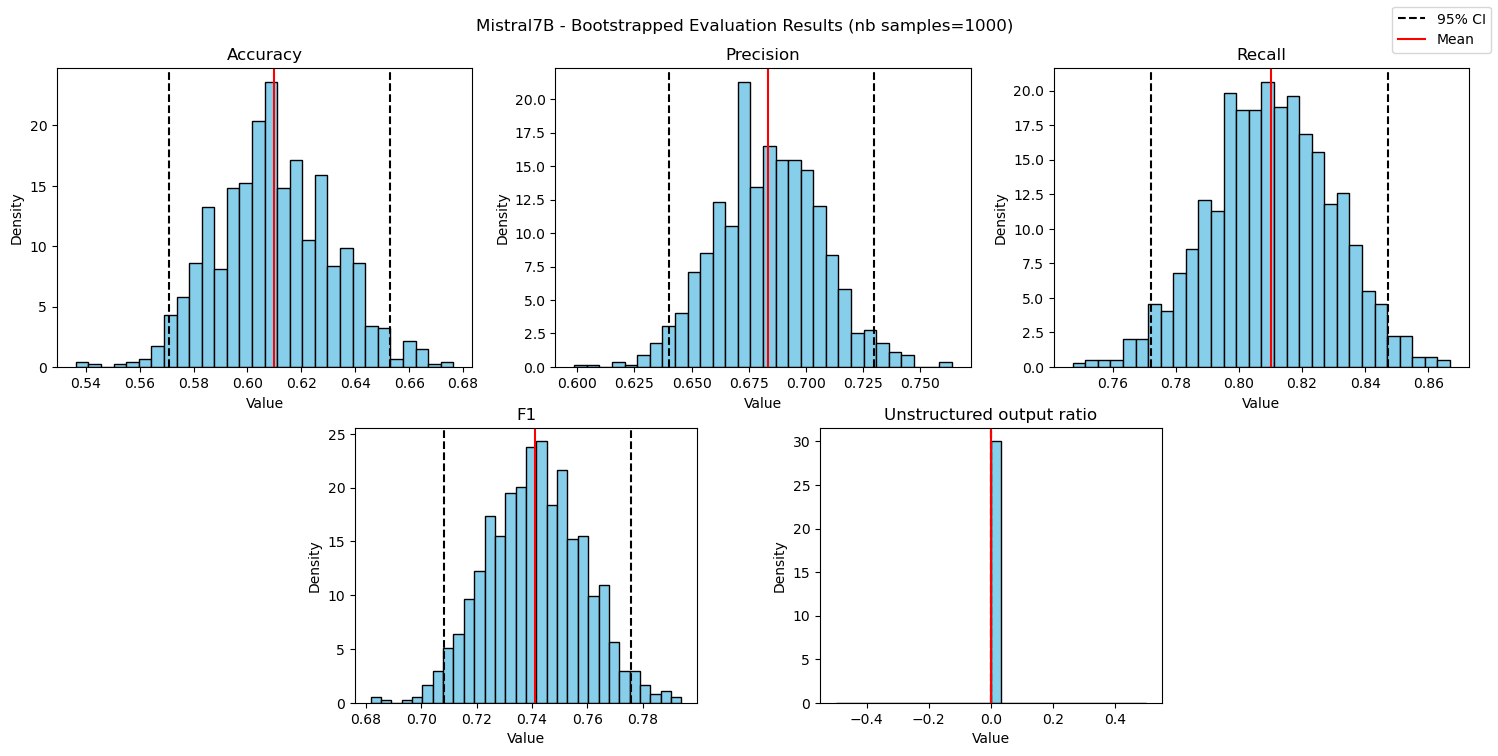
\includegraphics[width=\linewidth]{images//mistral//binary/mistral7b.png}
    \caption{Evaluation results for Mistral 7b on a binary task}
    \label{fig:enter-label}
\end{figure}

\begin{figure}[h]
    \centering
    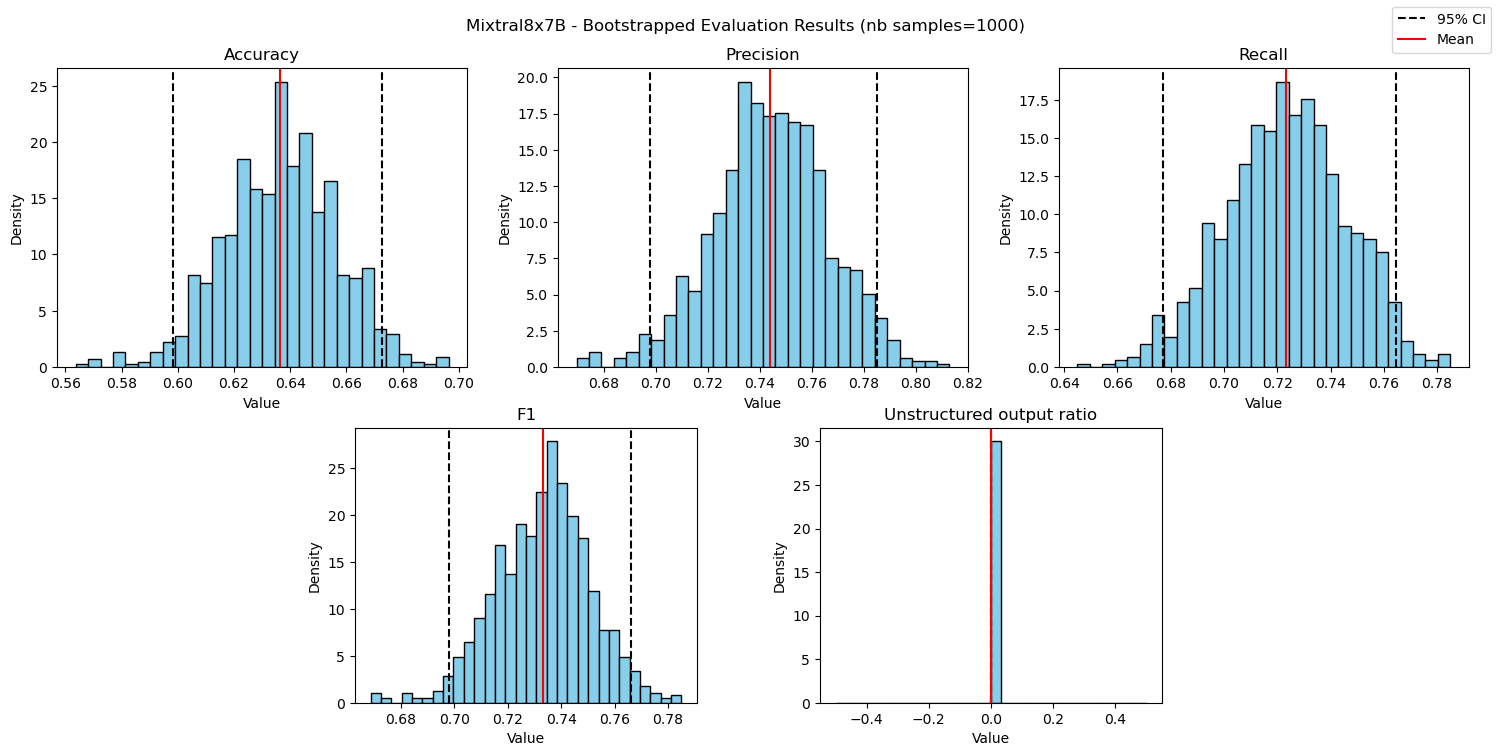
\includegraphics[width=\linewidth]{images//mistral//binary/mistral8x7b.png}
    \caption{Evaluation results for Mixtral 8x7b on a binary task}
    \label{fig:enter-label}
\end{figure}

Their comparative performance can be summarized in the table and graph below.

\begin{table}[h]
    \centering
    \resizebox{\columnwidth}{!}{%
    \begin{tabular}{c||c|c|c|c|c}
        Model & Accuracy & Precision & Recall & F1 Score & Unstructured output ratio \\
        \hline
        \hline
        Mistral 7b & 0.61 (0.5709-0.6527) & 0.6836 (0.6402-0.7297) & 0.8101 (0.7722-0.8472) & 0.7413 (0.7083-0.7757) & 0.0 (0.0-0.0)\\
        \hline
        Mistral 8x7b & 0.6365 (0.5982-0.6728) & 0.7439 (0.6977-0.7852) & 0.7232 (0.677-0.7645) & 0.7332 (0.6981-0.7661) & 0.0 (0.0-0.0)\\
    \end{tabular}%
    }
    \caption{Binary task: comparing Mistral 7b and Mixtral 8x7b}
    \label{tab:my_label}
\end{table}

\begin{figure}[h]
    \centering
    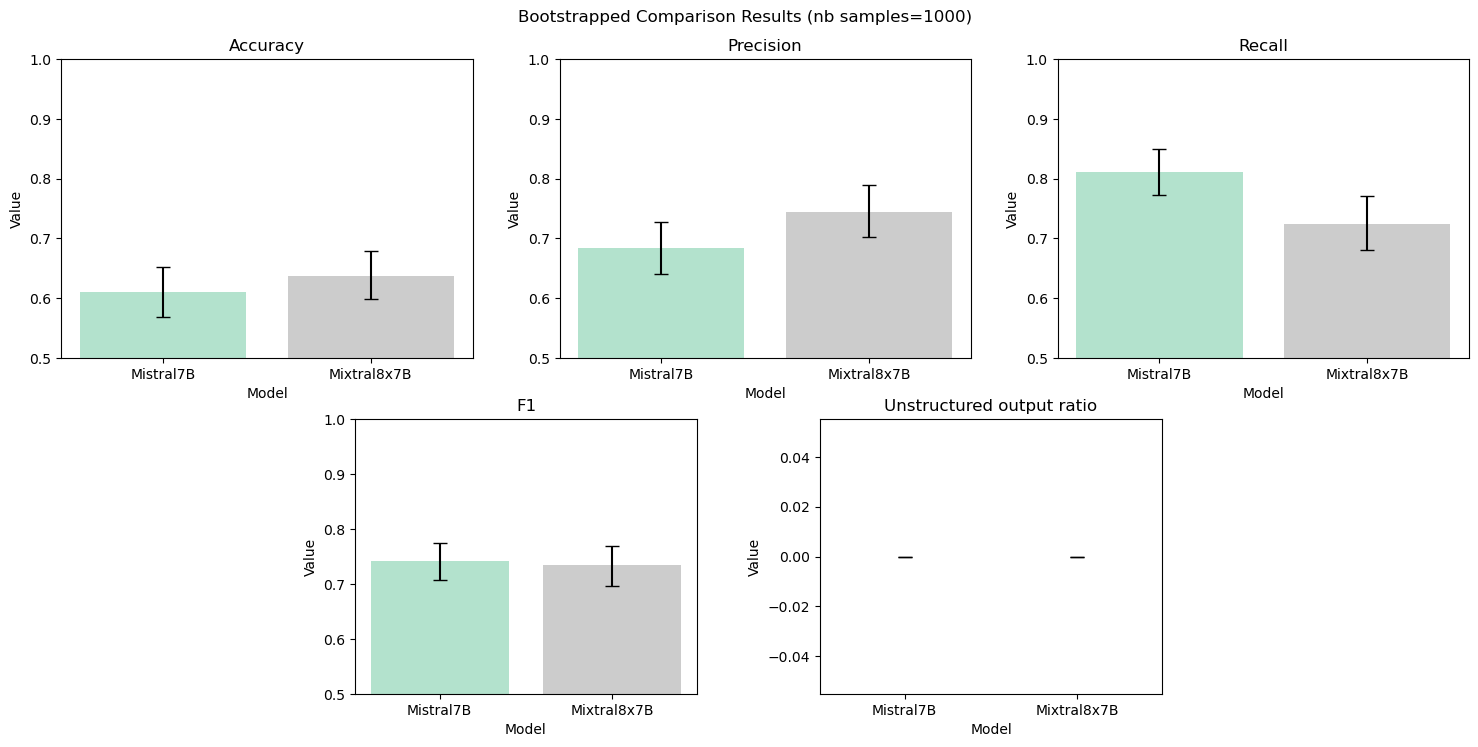
\includegraphics[width=\linewidth]{images//mistral//binary/comparison.png}
    \caption{Comparing Mistral 7b and Mixtral 8x7b on a binary task}
    \label{fig:enter-label}
\end{figure}

\newpage

We can draw several conclusions from these results. While there is no statistically significant difference in the accuracies or f1 scores, Mixtral 8x7b is slightly more precise than Mistral 7b, but has a lower recall. If the objective is to minimize the number of false positives, Mixtral 8x7b will be the better choice, while if we want to minimize the number of false negatives, Mistral 7b offers a better performance.
Both models were able to generate structured outputs for every sample.\\

To understand the weaknesses of both these models, we can analyze the errors that are made by each model. They do not seem to be linked to the document source (source\_x in the table). However, we can see an interesting trend when plotting the context length distributions:\\


\begin{figure}[h]
    \centering
    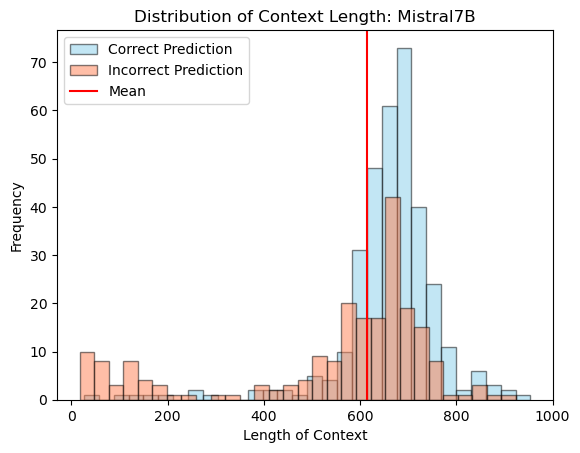
\includegraphics[width=0.45\linewidth]{images//mistral//binary/mistral7b_context.png}
    \caption{Context length distribution for Mistral 7b}
    \label{fig:enter-label}
\end{figure}

\newpage

\begin{figure}[h]
    \centering
    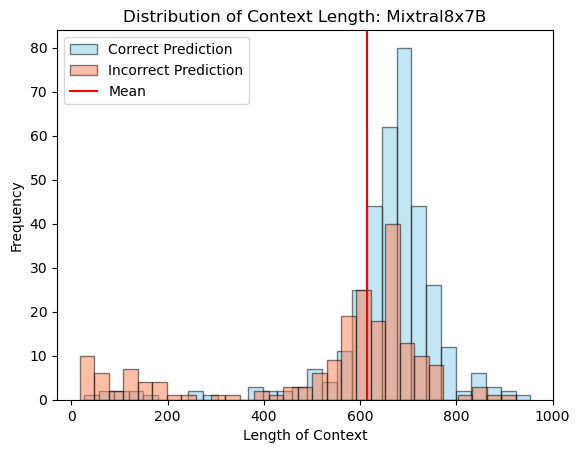
\includegraphics[width=0.45\linewidth]{images//mistral//binary/mistral8x7b_context.png}
    \caption{Context length distribution for Mixtral 8x7b}
    \label{fig:enter-label}
\end{figure}

For both models, the number of incorrect predictions largely surpasses the number of correct predictions below 300 tokens. This shows that both models have difficulties extracting information from short contexts. It is interesting to note that this trend is slightly more visible with the Mistral 7b model, most likely because it does not have as many parameters as Mistral 8x7b.\\

By examining the model results, we can also extract some patterns of failure:

\begin{itemize}
    \item Short contexts with a lot of affirmative words tend to trick the model: \textit{P: OK yeah, that sounds great. Thank you. D: Yeah, no problem.} - triggers a positive prediction.
    \item Implied symptoms also trigger false positives: \textit{[...] any other questions that you have? P: No, just hoping to get an answer to whatever is going on. D: OK, well at this point I will do a quick physical exam. [...]}. In this context, it is clear that the patient is experiencing symptoms, although they are not mentioned.
    \item Symptoms are mentioned, but they don't apply to the patient: \textit{[...] my grandfather had lung cancer [...]} is labeled as positive.
\end{itemize}

As well as anomalies that seem to be linked to the dataset:

\begin{itemize}
    \item Explicit symptoms are mentioned, but not labeled as symptoms in the dataset: \textit{[...] I can't move it at all. D: Alright, so um, it sounds like you have a shoulder dislocation. [...]}
    \item The patient does not experience any symptoms, but labeled as positive in the dataset.
\end{itemize}

The anomalies that were found during error interrogation are reported in the file \textbf{anomalies.txt}, in the root of the github repository.

\subsection{Multi-label Classification}

We can also run similar experiments on a multi-label classification task, where the objective is to determine the presence or absence of each of the following symptoms: (anxiety, concentration problems, constipation, cough, diarrhea, fatigue, fever, headache, nausea, numbness and tingling, pain, poor appetite, rash, shortness of breath, troubled drinking fluids, vomiting, other).

This is done using the following prompt:\\

\textit{For each symptom in symptom list return True if present and False if absent from the transcript. All symptoms required. Symptom list: 'anxiety', 'concentration problems', 'constipation', 'cough', 'diarrhea', 'fatigue', 'fever', 'headache', 'nausea', 'numbness and tingling', 'pain', 'poor appetite', 'rash', 'shortness of breath', 'trouble drinking fluids', 'vomiting', 'other'}\\

\begin{figure}[h]
    \centering
    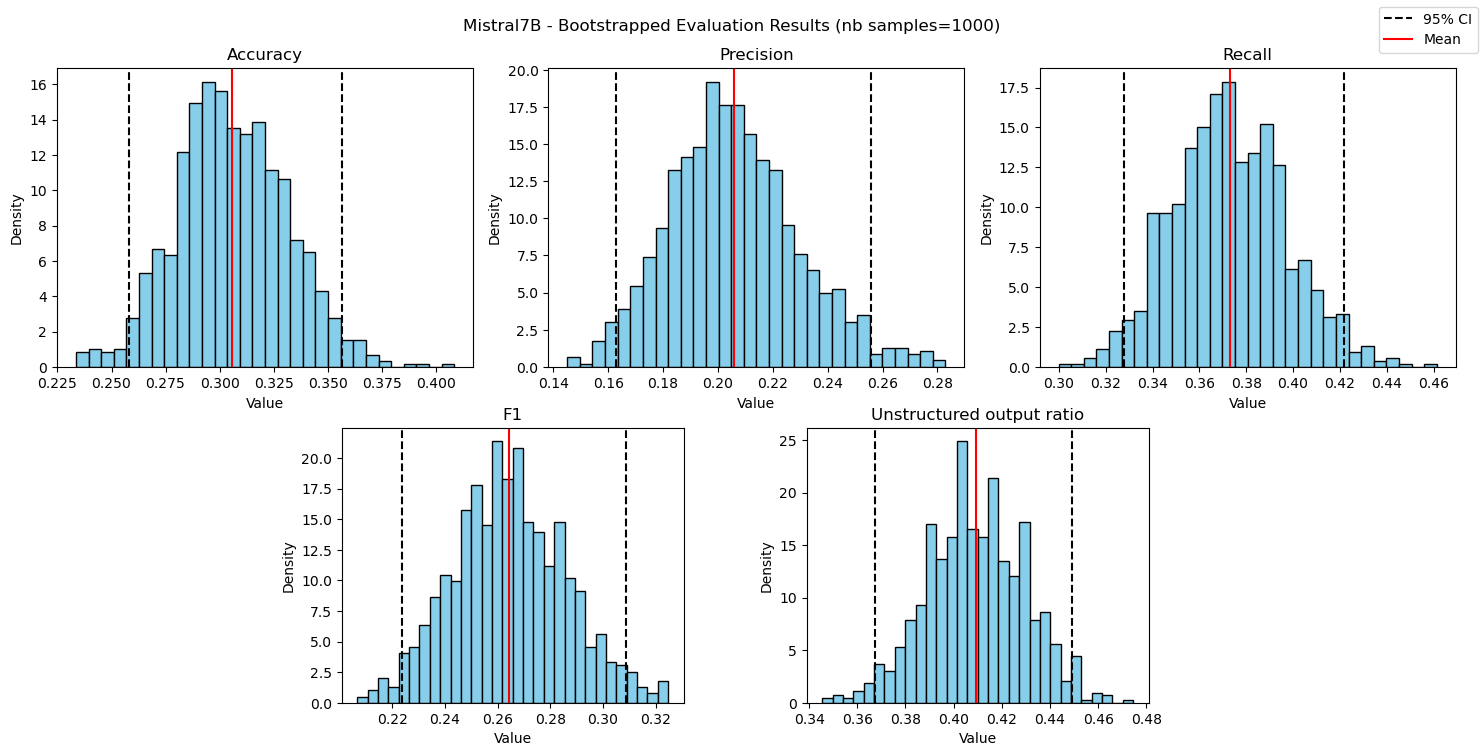
\includegraphics[width=\linewidth]{images//mistral//multilabel/mistral7b.png}
    \caption{Evaluation results for Mistral 7b on a multi-label task}
    \label{fig:enter-label}
\end{figure}

\begin{figure}[h]
    \centering
    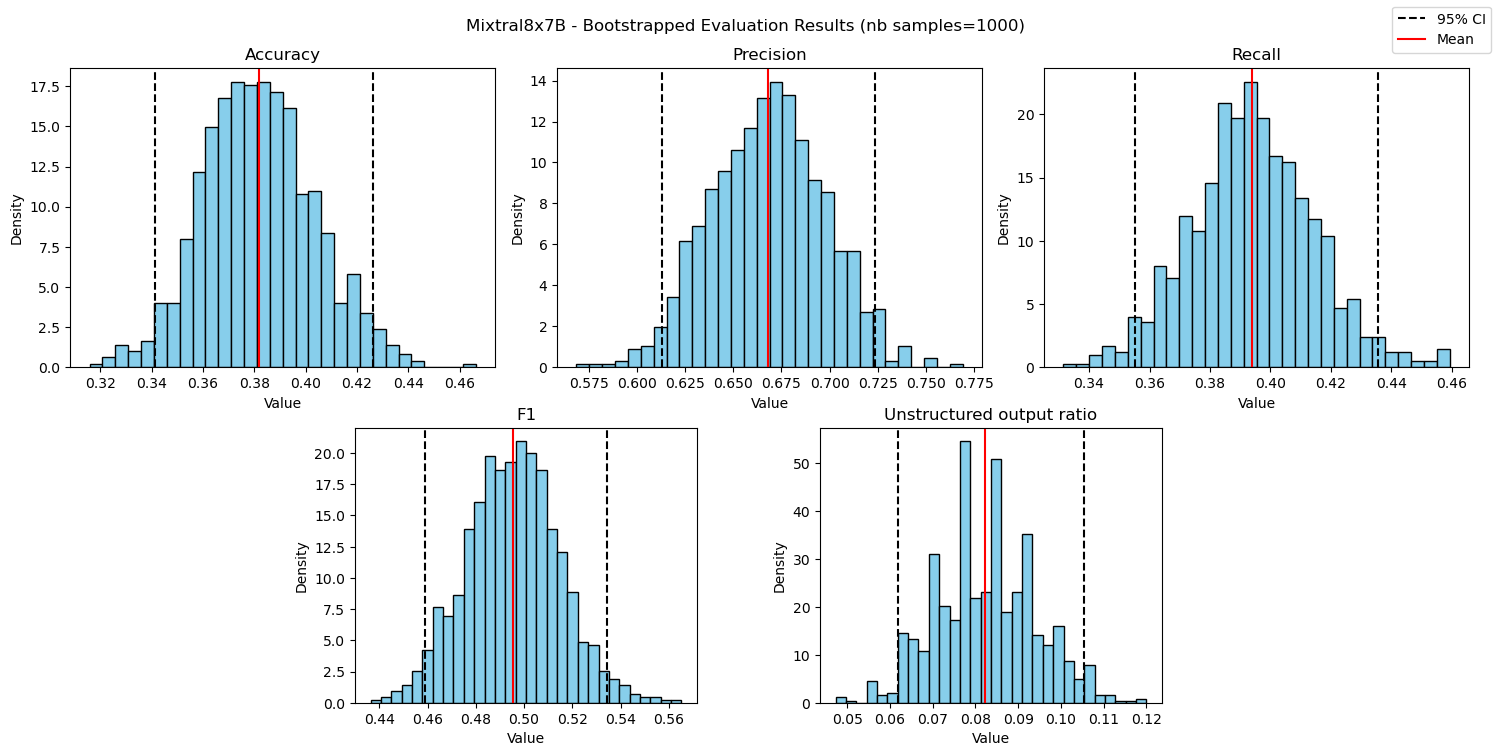
\includegraphics[width=\linewidth]{images//mistral//multilabel/mixtral8x7b.png}
    \caption{Evaluation results for Mixtral 8x7b on a multi-label task}
    \label{fig:enter-label}
\end{figure}

Their comparative performance can be summarized in the table and graph below.

\newpage

\begin{table}[h]
    \centering
    \resizebox{\columnwidth}{!}{%
    \begin{tabular}{c||c|c|c|c|c}
        Model & Accuracy & Precision & Recall & F1 Score & Unstructured output ratio \\
        \hline
        \hline
        Mistral 7b & 0.3058 (0.2582-0.3567) & 0.2059 (0.163-0.2556) & 0.3729 (0.3279-0.4218) & 0.2645 (0.2238-0.3089) & 0.4091 (0.3673-0.4491)\\
        \hline
        Mistral 8x7b & 0.3818 (0.3413-0.4263) & 0.6682 (0.613-0.7238) & 0.394 (0.3552-0.4355) & 0.4953 (0.4588-0.5345) & 0.0821 (0.0618-0.1055)\\
    \end{tabular}%
    }
    \caption{Multi-label task: comparing Mistral 7b and Mixtral 8x7b}
    \label{tab:my_label}
\end{table}

\begin{figure}[h]
    \centering
    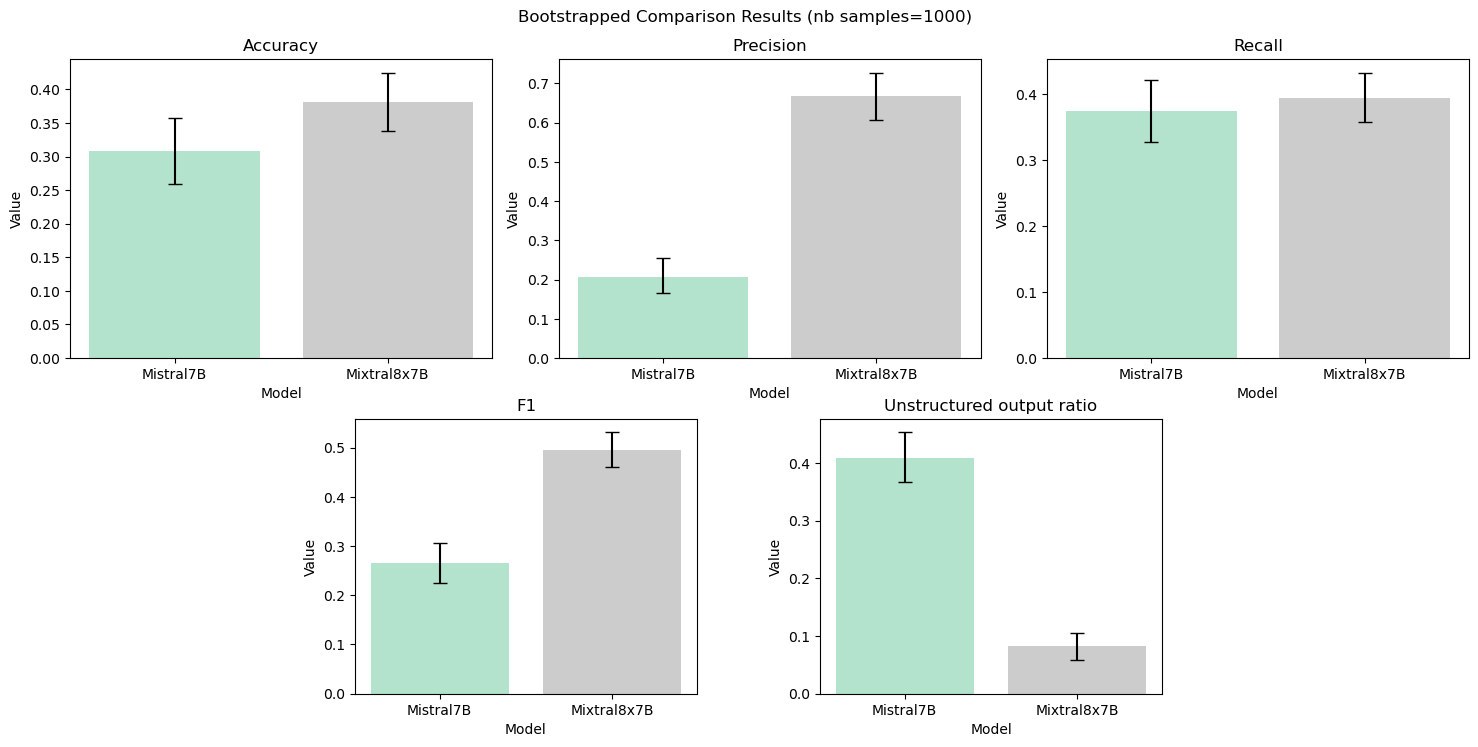
\includegraphics[width=\linewidth]{images//mistral//multilabel/comparison.png}
    \caption{Comparing Mistral 7b and Mixtral 8x7b on a multi-label task}
    \label{fig:enter-label}
\end{figure}

This time, the results between Mistral 7b and Mixtral 8x7b are much more visible, especially when looking at metrics such as Precision and F1 score. All these metrics do not take into account the unstructured outputs, but we can see that Mistral 7b produced almost 50\% of unstructured outputs, while only about 10\% of Mixtral 8x7b's outputs are unstructured. It is likely that these performances could be improved with prompt engineering.

\section{Assessing the performance of Llama 2 70b Chat}

Since there is no function calling mode with Llama 2, we need to implement an extraction mechanism to extract the answer from the model's output. This mechanism differs based on if the task is binary or multi-label classification, and will be detailed in each of the subsections.\\

After implementing the module for Llama 2 70b Chat in the code base, we can use the existing pipeline to produce our results. Similarly to what has been done in the previous section, we use bootstrapping to estimate the various metrics.

\subsection{Binary Classification}

To extract the information from the model's output, we experiment with different prompts. When the prompt finishes with the question "Are any medical symptoms mentioned in the transcript?", the model starts its answer with Yes or No. We therefore extract the first word from the output and map it to a boolean value. This method works surprisingly well, especially when associated with retries. Several prompts had an unstructured output ratios of zero, and most of the prompts had an unstructured output ratio around 1\%.\\

In order to achieve the highest possible performance, we use an iterative approach to improve the prompts. The log of the different prompts attempted can be found at the root of the github repo, under the name \textbf{prompt\_testing\_log.txt}. This document gives metrics for each of the prompts, as well as the reasoning behind each iteration. Since the log is rather long, we don't include it in this report, and focus on the best performing prompt.\\

The best results are obtained with the following prompt:\\

\textit{prompt = "You are a helpful model diagnosing diseases based on Doctor - Patient conversations. Given a conversation, you should determine whether the patient has symptoms or not. Some symptoms will be mentioned but will not apply to the patient. It is important that you only consider symptoms that are experienced by the patient. An example of a patient mentioning a symptom that does not apply to them is: 'P: My daughter is having fevers and barely sleeps'. Your answer should be 'No'. It is also important that you only consider explicit mentions of symptoms. An example of a patient not explicitly mentioning a symptom is: 'D: You need to get an MRI as soon as possible. P: OK. D: Alright.' Your answer should be: 'No'. You should refrain from answering yes if you are not certain. If you are not certain, your answer should be: 'No'. Are any medical symptoms mentioned in the transcript?"}\\

In this prompt, we address two failure points of the model (that were mentioned in the Mistral section): symptoms that are mentioned that don't apply to the patient, and symptoms that are implicit.\\

This prompt yields the following results for Llama 2 70b Chat:\\

\begin{figure}[h]
    \centering
    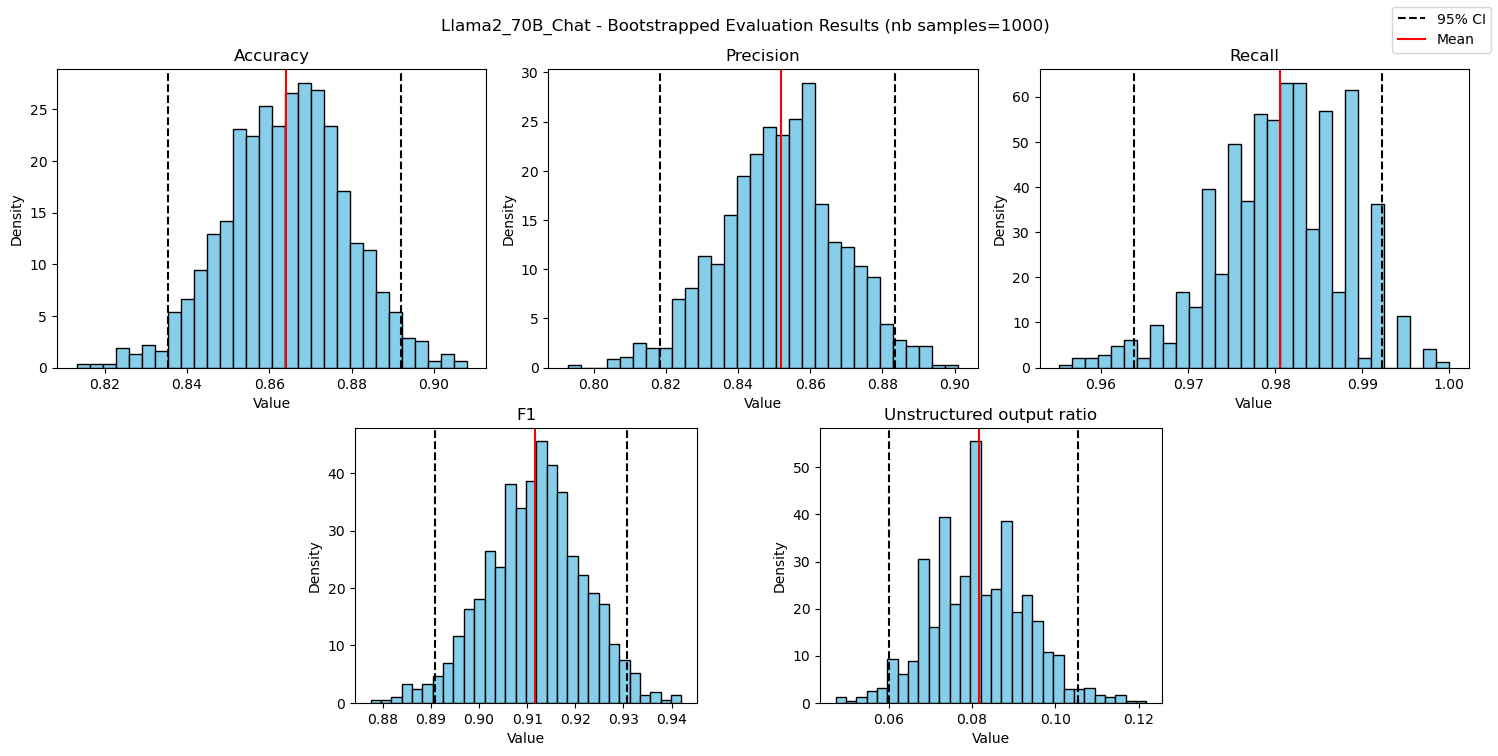
\includegraphics[width=\linewidth]{images/llama2/binary/prompt_8/llama2.png}
    \caption{Evaluation results for Llama 2 70b Chat on a binary task}
    \label{fig:enter-label}
\end{figure}

Its performance can be summarized in the table below: \\

\begin{table}[h]
    \centering
    \resizebox{\columnwidth}{!}{%
    \begin{tabular}{c||c|c|c|c|c}
        Model & Accuracy & Precision & Recall & F1 Score & Unstructured output ratio \\
        \hline
        \hline
        Llama 2 70b chat & 0.8634 (0.834-0.8916) & 0.8508 (0.8173-0.8834) & 0.981 (0.9657-0.9944) & 0.9112 (0.8901-0.9305) & 0.0821 (0.0618-0.1037)\\
    \end{tabular}%
    }
    \caption{Binary task: evaluating Llama 2 70b chat}
    \label{tab:my_label}
\end{table}

We obtain significantly higher metrics compared to the Mistral models. However, this comes at the cost of a larger unstructured output ratio. Other prompts can offer a lower unstructured output ratio for a slightly lower performance.\\

We can compare these results with the two Mistral models using the same prompt.\\

\begin{figure}[h]
    \centering
    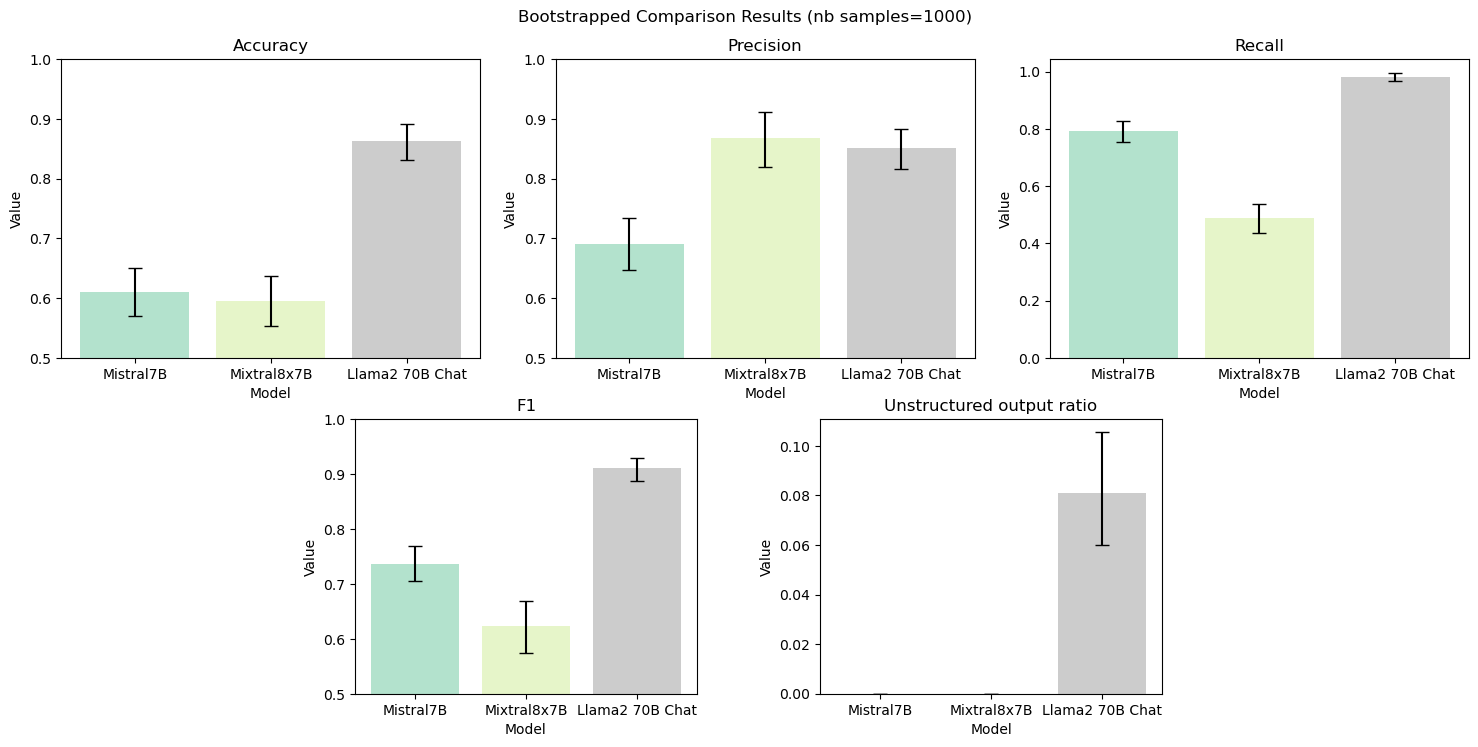
\includegraphics[width=\linewidth]{images/llama2/binary/prompt_8/comparison.png}
    \caption{Comparing Llama 2 70b chat with the two Mistral models - binary task}
    \label{fig:enter-label}
\end{figure}

This confirms our observation that Llama 2 70b chat significantly outperforms the two Mistral models (except for the precision metric). Interestingly, the Mistral models do not see a gain in performance with this optimized prompt.\\

\begin{figure}[h]
    \centering
    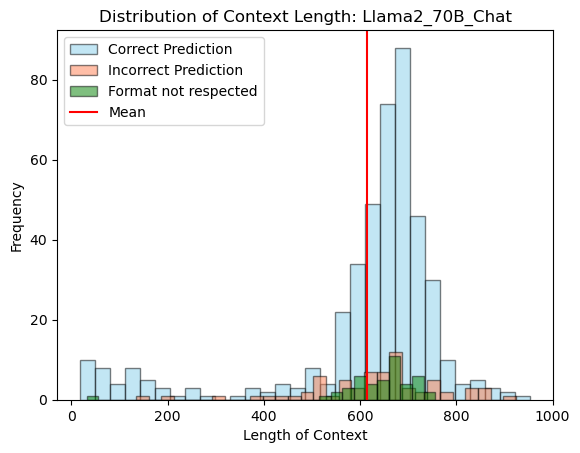
\includegraphics[width=0.45\linewidth]{images/llama2/binary/prompt_8/llama2_context_length.png}
    \caption{Context length distribution for Llama 2 70b chat - binary task}
    \label{fig:enter-label}
\end{figure}

The failure modes for this prompt are similar to the ones observed with Mistral models. Testing various prompts shows that it is possible to achieve an even higher performance by passing the list of acceptable symptoms (from the multi-label task) to the prompt, but this leads to a very high unstructured output ratio. Overall, it seems that past an F1 Score of about 90\%, increasing performance necessarily means increasing the unstructured output ratio.\\

This phenomenon is likely due to potential anomalies in the dataset, as mentioned previously. A non-negligible part of the samples seem to be mislabeled. It is therefore possible that models can only exhibit a higher performance by generating unstructured outputs, since those are not taken into account when computing the metrics. Please refer to the file \textbf{anomalies.txt} at the root of the github repository for examples of these anomalies.

\subsection{Multi-label Classification}

To implement multi-label classification, we need to use a different extraction mechanism for the model output. This can be done by prompting the model to generate JSON-like outputs. Since a large number of JSON outputs were used to train Llama, this method works relatively well with the following prompt:\\

\textit{You are a helpful assistant, that only communicates using JSON files. The expected output from you has to be a JSON file with the following structure:}\\

\textit{\{
    "Anxiety": bool (True or False),
    "Concentration\_Problems": bool (True or False),
    "Constipation": bool (True or False),
    "Cough": bool (True or False),
    "Diarrhea": bool (True or False),
    "Fatigue": bool (True or False),
    "Fever": bool (True or False),
    "Headache": bool (True or False),
    "Nausea": bool (True or False),
    "Numbness\_and\_Tingling": bool (True or False),
    "Pain": bool (True or False),
    "Poor\_Appetite": bool (True or False),
    "Rash": bool (True or False),
    "Shortness\_of\_Breath": bool (True or False),
    "Trouble\_Drinking\_Fluids": bool (True or False),
    "Vomiting": bool (True or False),
    "Other": bool (True or False)
\}}\\

\textit{Given a transcript, you have to return a JSON file with the presence of each symptom in the transcript. 
For instance, given the following transcript: 'D: And are you feeling better? P: No, I'm not. I'm still 
not very hungry and need to sleep all the time.' you should return:}\\

\textit{\{
    "Anxiety": false,
    "Concentration\_Problems": false,
    "Constipation": false,
    "Cough": false,
    "Diarrhea": false,
    "Fatigue": true,
    "Fever": false,
    "Headache": false,
    "Nausea": false,
    "Numbness\_and\_Tingling": false,
    "Pain": false,
    "Poor\_Appetite": true,
    "Rash": false,
    "Shortness\_of\_Breath": false,
    "Trouble\_Drinking\_Fluids": false,
    "Vomiting": false,
    "Other": false
\}
}\\

The idea for this prompt format was found on \href{https://www.reddit.com/r/LocalLLaMA/comments/15742zf/comment/jt4ag66/?utm_source=share&utm_medium=web3x&utm_name=web3xcss&utm_term=1&utm_content=share_button}{this reddit post}.\\

\newpage

\begin{figure}[h]
    \centering
    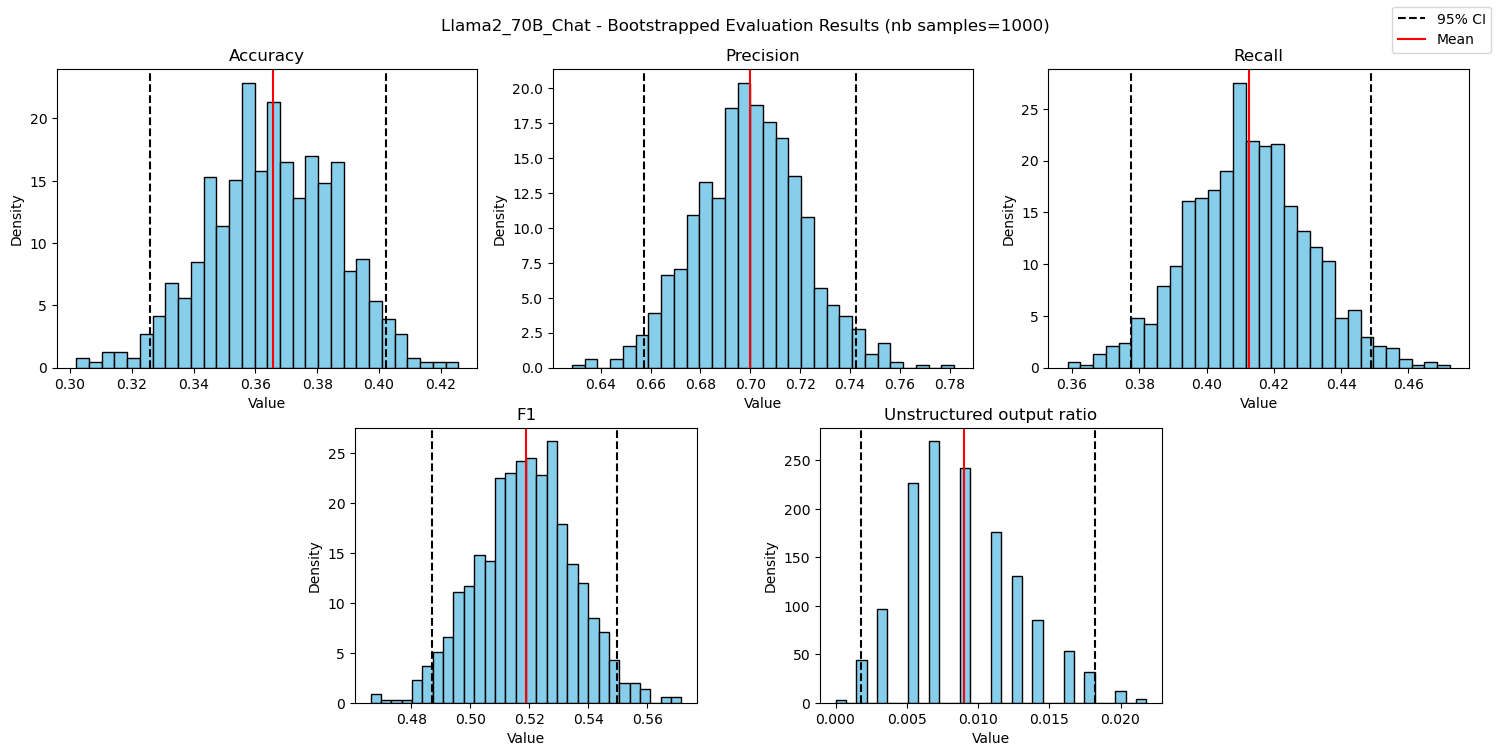
\includegraphics[width=\linewidth]{images/llama2/multilabel/llama2.png}
    \caption{Evaluation results for Llama 2 70b Chat on a multi-label task}
    \label{fig:enter-label}
\end{figure}

The performance is much lower compared to the binary task, and could most likely be improved with prompt engineering. However, the unstructured output ratio is very low with an average of only 0.9\%.

\begin{figure}[h]
    \centering
    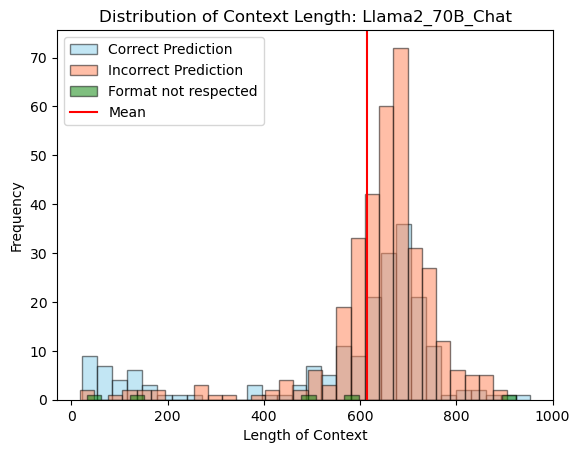
\includegraphics[width=0.45\linewidth]{images/llama2/multilabel/llama2_context_length.png}
    \caption{Context length distribution for Llama 2 70b chat- multi-label task}
    \label{fig:enter-label}
\end{figure}


\section{Possible Improvements}

Given more time, it would have been interesting to perform prompt engineering on the multi-label task as well to assess the performance of all three models, and see if it is possible to reach a similar performance to their binary counterparts.\\

Regarding the output generation for Llama 2: some frameworks such as LMQL offer interesting approaches to structured output generation, almost similar to function calling. I tried to implement it, but it does not seem to be compatible with the Together AI API. However this would be very pertinent in the context of a model running locally.\\

Some improvements could also be made on the code base. For instance, the current API rate limit exception catcher is the same as the unstructured output exception catcher, although these two exceptions should be handled differently - there is no need for an exponential backoff if the output is unstructured, the pipeline should generate a new output without waiting. Another possible improvement is modifying the parallelized implementation to have each worker start with an offset. The current implementation most likely reaches the API rate limit, as all workers attempt to generate an output at the same time, leading to unnecessary overhead.\\


\end{document}
